\documentclass[11]{article}
\usepackage{graphicx}
\graphicspath{{images/}}


\title{CS2002 Practical 4 - \\Stable Circuits}
\date{11/04/2018}
\author{Matriculation Number: 160001362}

\begin{document}
	
	\maketitle
	\newpage
	\tableofcontents
	
	\newpage
	\section{Overview}
	This practical specified the development of a system to 
	\section{Design and Implementation}
		The index based implementation is contained with a folder 'Index\_Based' and the pointer based implementation is contained within a folder 'Pointer\_Based', both of which are within the 'ReadMyMind' directory. The code is heavily commented to make it clearn how each of the implementations work. \\\\Both implementations of the program have the same following files within their respective directories:
		\subsubsection{Files and Libraries}
				\begin{itemize}
					\item \textbf{readmymind.c} - This file contains the main function of the program. It is responsible for handling the control flow of the program and declaring the necessary structs and variables required.
					\item \textbf{cards.c} - This file is responsible for initialising the fundamental data structures required for use in the program including the deck, the cards, as well as the columns used to store the 21 cards (using getDeck, getCard, and fill respectively).
					\item \textbf{io.c} - Handles the input and output of the solution. The file contains functions to get the user's column selection, validate this input, and convert this input into an integer format more easily utilised in the program. In addition the file contains a function to print the cards of a columns structure to the terminal as well as print the centre card of a columns structure.
					\item \textbf{actions.c} - Contains functions relating to the actions performed during the card trick. The 'gather' function creates a new columns struct and initialises it with the previous columns rearranged so that the column selected by the user is in the centre. The 'deal' function iterates through the cards of each column in the columns struct returned from 'gather' and deals the cards into the new struct from left to right across the columns.
					\item \textbf{readmymind.h} - Contains definitions for the size of data structure dimensions (e.g. COLUMN\_SIZE, SUIT\_SIZE), the structs representing the data structures, as well as for the signatures of functions used throughout the program.
					\item \textbf{stdbool.h} - Used to allow true and false values to be returned when validating the user's input.
					
					\item \textbf{stdlib.h} - Used to set appropriate values to NULL as well as enabling the use of malloc and free.
					
					\item \textbf{stdio.h} - Used for input and output.
					
					\item \textbf{assert.h} - Used to terminate program if branches of code are reached that should be unreachable.
					
					\item \textbf{string.h} - Used for the strlen function to check if the size of the user's input is greater than a single character. Although not explicitly stated as one of the permitted libraries in the specification, Dr Fayed stated in a query that its use is permissible:
					
					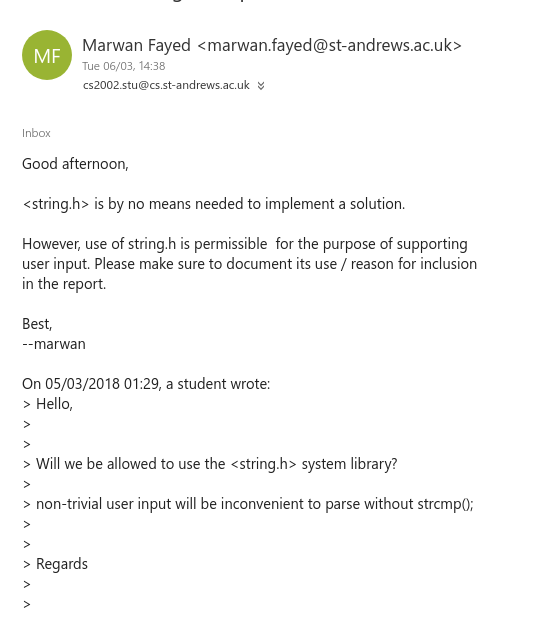
\includegraphics[scale=0.4]{Email.png}
				\end{itemize}
		\subsection{Index Based}
			\subsubsection{Summary}
			Declares and initialises a deck array of 52 cards and uses it to fill a Columns struct of 21 cards (of 3 column structs of 7). The columns are filled by randomly generating a number (signifying a card to select from the deck) and checking an array of selected values to see if the card has already been picked. It does this until 21 cards have been selected. \\\\The user then inputs their chosen column (this data is validated using an array of valid inputs) and this value is converted to an integer format and is then used to gather the columns. The columns are gathered by assigning the selected column of the previous Columns struct to the middle Column struct of the new Columns struct. The other columns are then iterated over and assigned. \\\\Finally the Columns struct with the selected column in the middle is dealt to a new set of columns by iterating over each element in the new Columns struct and calculating which old element should be dealt. \\\\The above process of getting user input, gathering the cards, and dealing the cards is then repeated three times with the user's card being displayed at the end.
			\subsubsection{Data Structures}
				\begin{itemize}
					\item \textbf{Card} - Has two integer attributes:
						\begin{itemize}
							\item \textbf{suit} - a number from 0 - 3 representing either spade, heart, diamond, or club.
							\item \textbf{rank} - a number from 0 - 12 representing and Ace, 2, 3, 4, 5, 6, 7, 8, 9, Jack, Queen, or King respectively.
						\end{itemize}
					
					\item \textbf{Deck} - Has one attribute 'cards' which is an array of type Card which has the size of the constant DECK\_SIZE (in the general case 52).
					
					\item \textbf{Column} - Like the Deck struct - has one attribute 'cards' which is an array of type Card which has the size of constant COLUMN\_SIZE (typically 7).
					
					\item \textbf{Columns} - Has an attribute 'column' which is an array of columns of size NUM\_COLUMNS (typically 3).
				\end{itemize}
		\subsection{Pointer Based}
			\subsubsection{Summary}
			The pointer based implementation has an additional C file '\textbf{linkedlist.c}' which has functions to interface with the linkedlist data structure declared in readmymind.h. These include functions to create and add nodes to a linked list as well as retrieve nodes from a linked list. In addition there is a function to free the memory occupied by nodes of a linked list to avoid memory leakage and a function to update the indices of a given linked list. \\\\A linked list implementation by HackerEarth\footnote{https://www.hackerearth.com/practice/data-structures/linked-list/singly-linked-list/tutorial/} was used to give an idea of how to implement a basic linked list data structure in C. \\\\ The pointer version uses almost the exact same process as described in section 2.1.1. Aside from the way the data structure is accessed during the trick, the main difference between the two implementations is the way that the user input and output works. In the pointer based implementation instead of accessing card icons to be displayed using a constant array, a switch statement containing print statements is used. \\\\Similarly, instead of storing a constant array of valid inputs and accessing it to validate the user's input, a switch statement is used for input validation. A switch statement rather than iteration is also used in the gather stage. While the implementation of these features is more elegant in the array based implementation, this alternate implementation demonstrates that arrays are not strictly necessary.
			\\\\The pointer implementation shares a common Card struct with the index based implementation, however the other following structures differ in implementation:
			\subsubsection{Data Structures}
				\begin{itemize}
					\item \textbf{Card} - Has two integer attributes:
						\begin{itemize}
							\item \textbf{suit} - a number from 0 - 3 representing either spade, heart, diamond, or club.
							\item \textbf{rank} - a number from 0 - 12 representing and Ace, 2, 3, 4, 5, 6, 7, 8, 9, Jack, Queen, or King respectively.
						\end{itemize}
						
					\item \textbf{LinkedList} - Has the following attributes: 
						\begin{itemize}
							\item \textbf{card} - Stores a Card attribute that can be thought of as the 'value' of the node (a card in the deck or columns).
							\item \textbf{next} - A linkedlist pointer to the next node the in the list.
							\item \textbf{index} - An integer signifying a node's position in its linkedlist - manually set and used so that it would be easier to translate the functions in the index/array based implementation into the pointer implementation.
							
							\item \textbf{chosen} - A boolean used when selecting the random 21 cards from the deck of cards to signify whether a particular card has already been selected.
						\end{itemize}
						
					\item \textbf{Node} - A typedef that allows a LinkedList pointer to be declared using the keyword 'Node'.										
					
					\item \textbf{Deck} - A struct that has one attribute 'node' which is a LinkedList Node. Used to allow 52 nodes to be added, each of which stores a unique playing card.
					
					\item \textbf{Columns} - A struct that contains three Node attributes called 'first', 'second' and 'third'. Each attribute stores the heads of their respective linkedlists which represent the three columns of the card trick.
				\end{itemize}
				
	\section{Testing}
		The following is a sample of output generated from testing the implementations. The function scanf was used to get the input from the user and proved surprisingly robust given the limited scope of this program.
			\subsection{Input Validation}
				\begin{figure}[h!]
				
					\caption{Invalid inputs being validated. Includes multiple character input, character input larger than allocated memory for the input char*, invalid single character input, as well as some miscellaneous input.}
					\centering
					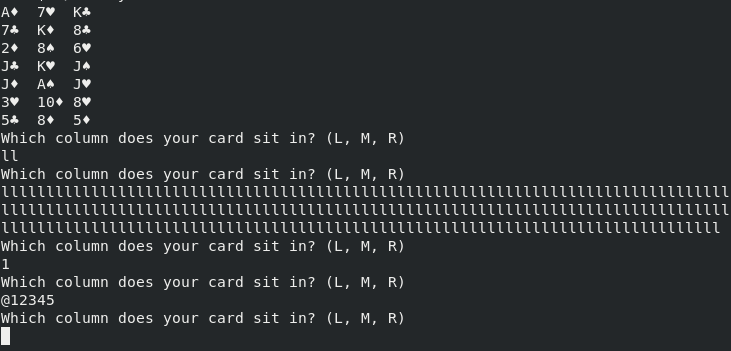
\includegraphics[scale=0.45]{IndexInvalidInput.png}
				\end{figure}
				
				\begin{figure}[h!]
					\caption{Example of valid inputs being accepted. Valid inputs include the characters l, L, r, R, m, and M.}
					\centering
					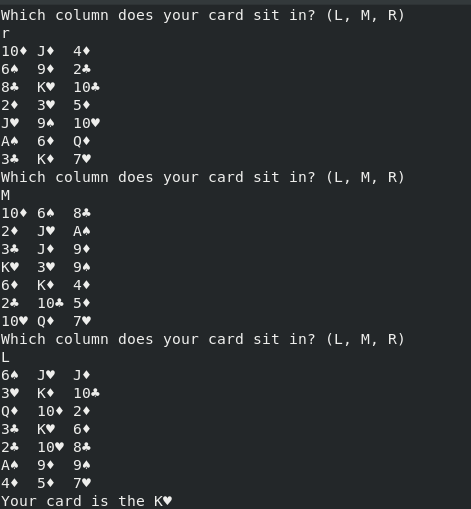
\includegraphics[scale=0.4]{IndexValidInput.png}
				\end{figure}
				
				\begin{figure}[h!]
					\caption{Example of valid inputs being accepted with preceding white space (white space and new line characters do not effect the single character input).}
					\centering
					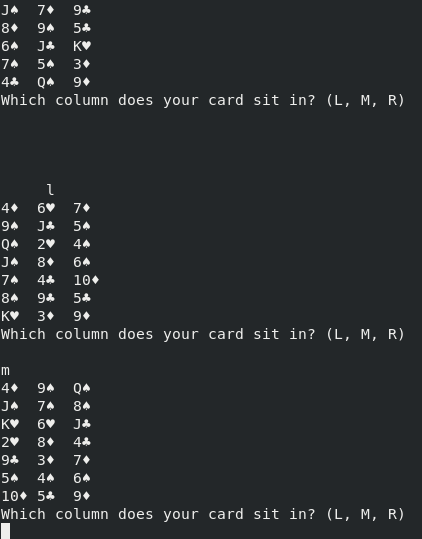
\includegraphics[scale=0.36]{IndexWhitespaceValid.png}
				\end{figure}
			
			\newpage \clearpage
			\subsection{Gathering Columns}
				\begin{figure}[h!]
					\caption{Output of the gather stage when the deal stage is commented out. The output shows that the correct centre column is assigned each time.}				\centering
					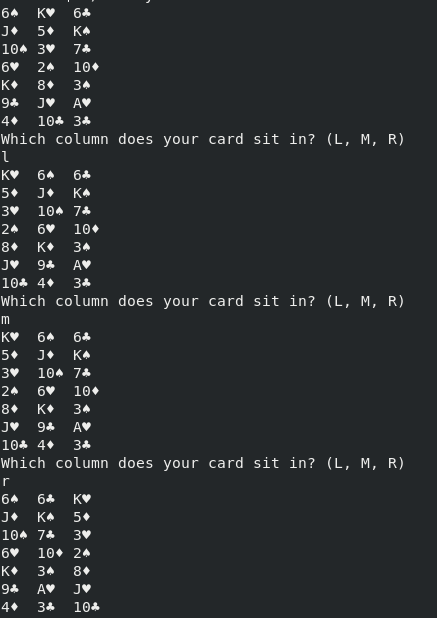
\includegraphics[scale=0.5]{Gather.png}
				\end{figure}
			
			\clearpage
			\subsection{Dealing Cards}
				\begin{figure}[h!]
					\caption{Output of multiple deal stages when the user's card is the 3 of spades. This output clearly shows that the cards are correctly dealt left-to-right, top-to-bottom.}				\centering
					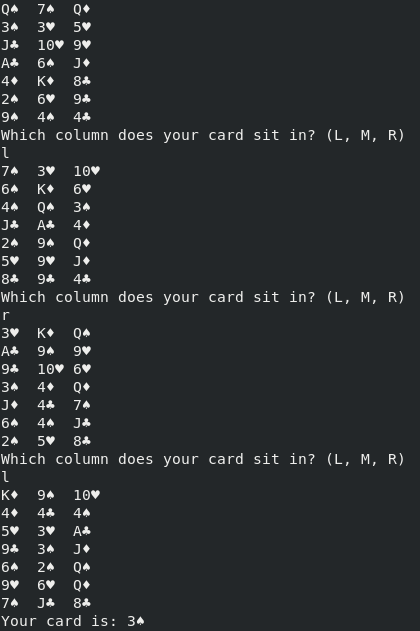
\includegraphics[scale=0.5]{Deal.png}
				\end{figure}
	\newpage
	\section{Conclusion and Evaluation}
	In conclusion the requirements specified in the practical document to develop a card trick program have been fully implemented using both an index based implementation as well as non-global pointer based solution utilising a linked list structure. The solutions also both follow the constraints specified in regard to the allowed libraries as well as both only using local instances of data structures. \\\\ To improve upon my solution I would re-implement the way the newColumns struct is initialised in the pointer implementation when the cards are gathered and dealt. The current implementation of the program leaks 1.5MB of memory due to unused allocated memory that was once pointed to by a Columns struct. Without the frees at the end of the main function the program initially had over 3MB of leaked memory. I attempted to free the original columns struct when newColumns is assigned in both the gather and deal functions to reduce the amount from 1.7MB to 0MB however this resulted in a segmentation fault and so I decided to permit some memory not being freed (this would be more of a problem if the trick is repeated many times).
	
				\begin{figure}[h!]
					\caption{Output of 'valgrind ./readmymind'}				\centering
					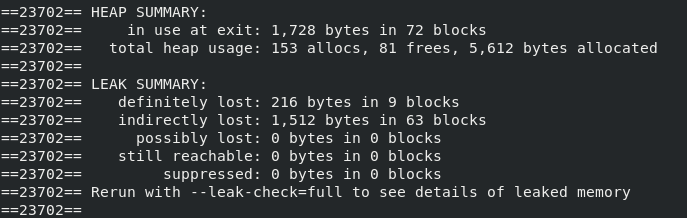
\includegraphics[scale=0.5]{ValGrind.png}
				\end{figure}
	
	
	\section{Extensions}
		\begin{itemize}
			\item \textbf{Allow Repetition of Trick} - In both implementations a while loop has been added to the main method to allow the user to repeat the card trick if they input the characters 'Y' or 'y' with anything else signifying an exit character. This has been achieved through the addition of a function getUserChoice in the io.c file which similarly to the getUserCol function gets the user's choice. A value of true is returned from a subsequent function isValidChoice if either character is entered.
				
			\item \textbf{Improve Ouput} - Improved output has been implemented with the letters A, J, Q, and K being output for the ranks 0, 10, 11 and 12 respectively and unicode card icons are output for the suits 0, 1, 2, and 3. For the suits 1 and 2 (hearts and diamonds) ANSI character codes have been used to display the suit icons in the colour red. \\\\
		
			\item \textbf{Complexity Discussion} - It seems counter-intuitive to use pointers and a linked list for such an application due the natural way in which an index based solution can represent cards in columns. In addition to this, linked lists typically take O(n) time to traverse to access an element where as arrays are constant time, O(1), access using an index. The main argument for using linked lists in any application is the ability to dynamically reallocate the size of the data structure utilising it however in this application we know from the start what size data structures (decks and columns) we will be working with.
		\end{itemize}
		
		\begin{figure}[h]
					\caption{Demonstration of repeating trick as well as improved output}				\centering
					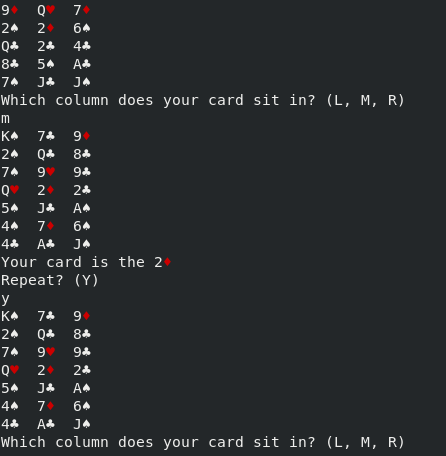
\includegraphics[scale=0.5]{Repeat.png}
		\end{figure}
			
			
		
	\begin{thebibliography}{1}
  		\bibitem{lit1} Mohd Sanad, Zaki Rizvi, \textit{"Singly Linked List Tutorial"}, HackerEarth, https://www.hackerearth.com/practice/data-structures/linked-list/singly-linked-list/tutorial/, (2016).
  	\end{thebibliography}
		
\end{document}